\chapter{Introducción}
\label{cap:intro}
%\chapterquote{Hablaban siempre de dinero y planeaban asaltar un banco}{Domingo Cavallo, 2001}


\subsection*{Convección Mixta}

Un fluido, en virtud de su masa y su velocidad, puede transportar momento. Además, en virtud de su temperatura, puede transportar calor. Estrictamente hablando, la convección es el transporte de energía debido al movimiento global de un medio. Sin embargo, en ingeniería es común utilizar el término convección de forma más amplia para describir la transferencia de calor desde una superficie hacia un fluido en movimiento cuando ambos están a diferentes temperaturas \cite{cengelheat,incropera}. 

La transferencia de calor por convección puede clasificarse según la naturaleza del flujo. Hablamos de convección forzada cuando el flujo es provocado por actores externos como puede ser la acción de bombeo o un gradiente de presión; en cambio, en la convección natural, el flujo es inducido por fuerzas boyantes o de flotación, las cuales se surgen debido a diferencias de densidad producidas por variaciones de temperatura en el propio fluido (Figura \ref{fig:natural_forzada}).

\begin{figure}[H]
 \centering
    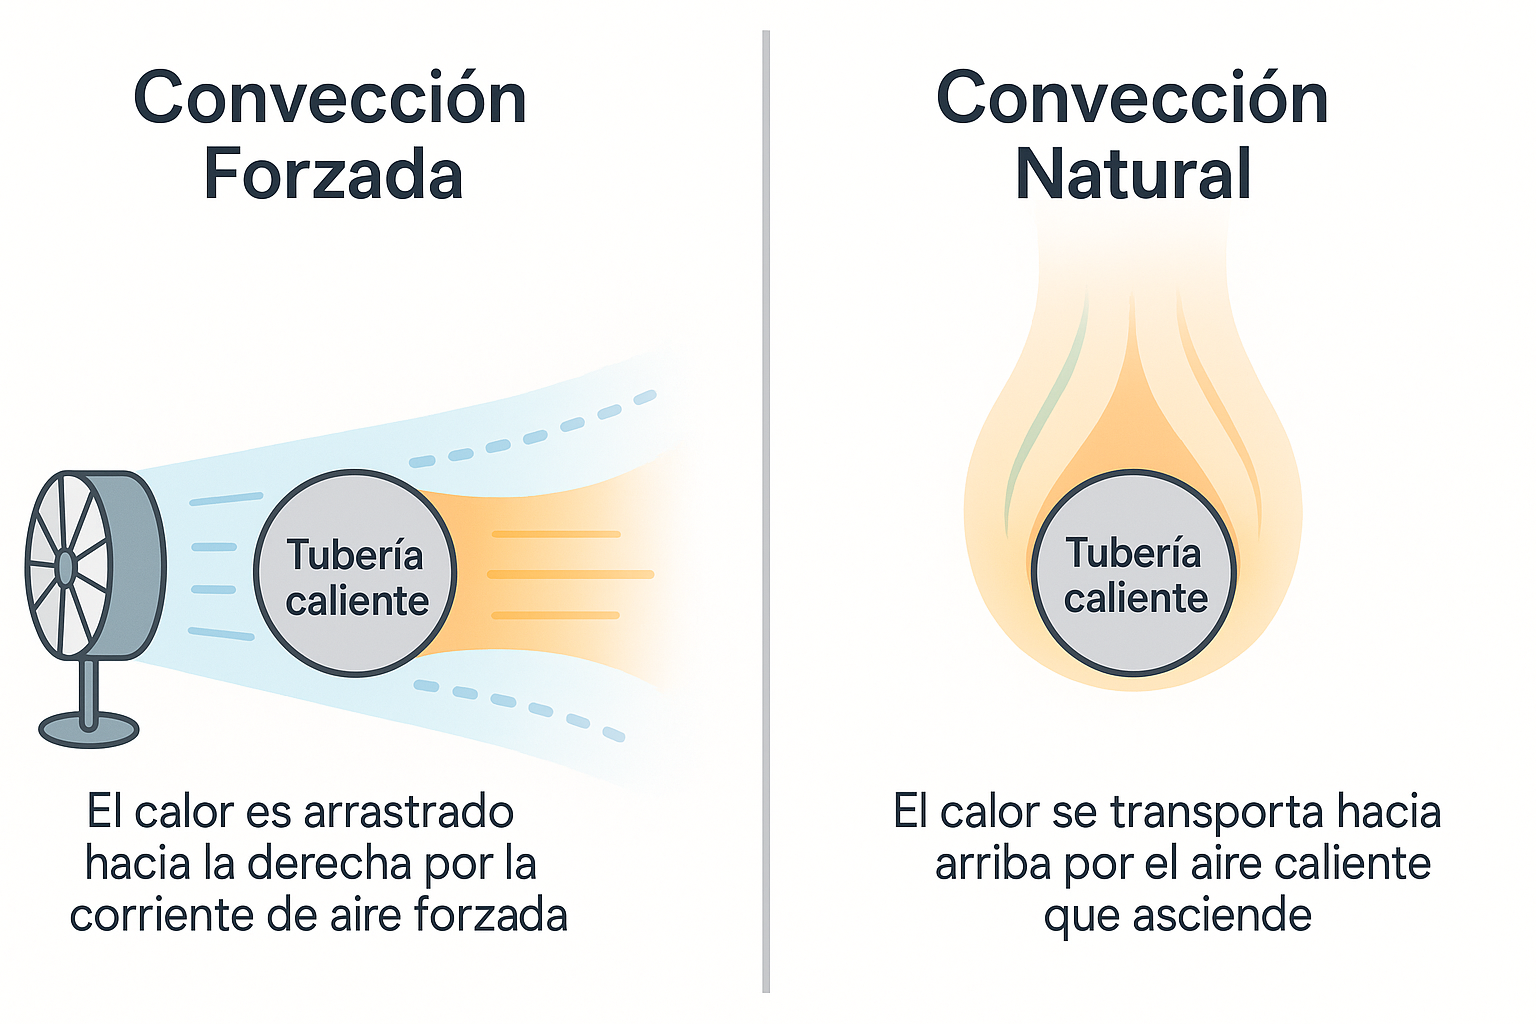
\includegraphics[width=0.6\textwidth]{figures/cap1/natural_forzada.png}
    \label{fig:natural_forzada} 
 \caption{Comparación esquemática de la transferencia de calor alrededor de una tubería caliente: (izquierda) convección forzada; (derecha) convección natural.} 
 \label{fig:natural_forzada}
\end{figure}

Los primeros estudios sobre la transferencia de calor por convección trataron las ramas de la convección forzada y la convección natural de forma separada, sin considerar la posible interacción entre ambas. Por un lado, los experimentos de Henri Bénard (1901) marcaron un hito en la comprensión de la convección natural \cite{benard1901}. Más tarde, Lord Rayleigh (1916) desarrolló la base teórica de la inestabilidad térmica en capas fluidas \cite{rayleigh1916}. En paralelo, en el ámbito de la convección forzada, trabajos como el de Dittus y Boelter (1930) establecieron correlaciones empíricas para la transferencia de calor en tubos \cite{dittus1930}. No fue sino hasta mediados del siglo XX que comenzó a reconocerse que ambos mecanismos pueden coexistir en muchas configuraciones de interés práctico. Así surgió el concepto de convección mixta, donde la convección forzada y la natural actúan simultáneamente como casos extremos de un fenómeno más general \cite{metais1964}. 

\subsection*{Régimen de Transición y Transición Laminar-Turbulenta}

Cuando un fluido se desplaza a través de un conducto o sobre una superficie, su movimiento puede clasificarse en dos tipos de régimen: laminar o turbulento \cite{white}. En el régimen laminar, el flujo es ordenado y las partículas del fluido se mueven en capas paralelas sin mezclarse entre sí. En cambio, en el régimen turbulento, el flujo es caótico, con remolinos, tiende a mezclarse, y presenta fluctuaciones en los campos de velocidad y presión \cite{kundu}. En ese sentido, un flujo que se encuentra en un estado desarrollado\footnote{Esto es, sus magnitudes no varían con el tiempo o con el espacio en un sentido estadístico.} intermedio, se dice que el flujo está en régimen de transición. Este estado de flujo no debe confundirse con la transición laminar-turbulenta del sistema, donde el flujo evoluciona de un régimen laminar a un régimen turbulento completamente desarrollado. Esta transición puede ocurrir en el tiempo (transición laminar-turbulenta temporal) o en el espacio (transición laminar-turbulenta espacial).

Por otro lado, la transición laminar-turbulenta es un fenómeno de gran importancia para la ingeniería y la física aplicada ya que está presente en diferentes dispositivos termohidráulicos. El cambio de un régimen a otro puede tener un impacto significativo en la transferencia de calor. El coeficiente de fricción (factor de Darcy) o el coeficiente de convección (numéro de Nusselt) se incrementan notablemente cuando se produce la transición \cite{incropera,white}. En ese sentido, el estado transitorio no es deseado desde el punto de vista ingenieril ya que es intermitente (es decir, el flujo puede fluctuar entre los regímenes laminar y turbulento), sin embargo, el estudio de la transición es relevante para poder controlar el fenómeno o anticipar, y por tanto aprovechar, su comportamiento. Por ejemplo, un problema importante se da en el diseño de intercambiadores de calor cuando el punto de trabajo del flujo dentro de los tubos o conductos se encuentra en régimen de transición donde las magnitudes relevantes (como coeficientes de fricción y de transferencia de calor) tienen una gran variación \cite{ghajar2019heat}.

La evolución de un flujo, tanto en el tiempo como en el espacio, depende de las perturbaciones externas que reciba (por ejemplo, cambios de presión o de temperatura), de las condiciones de borde a las que esté sometido (como puede ser la rugosidad, flujo de calor en las paredes o gradientes de presión, entre otros) y de la respuesta del propio sistema, determinada por sus propiedades físicas y el régimen de flujo. Para modelar matemáticamente las condiciones que pueden modificar ese régimen -es decir, los estados iniciales capaces de desencadenar una transición- y analizar cómo dicha transición impacta en la transferencia de calor, se recurre a la teoría de estabilidad hidrodinámica \cite{schmid}. Esta teoría ofrece un marco para predecir cuándo un flujo laminar se volverá inestable mediante el estudio de la evolución de pequeñas perturbaciones: si estas crecen en el espacio o en el tiempo, el flujo pierde su estabilidad y eventualmente transiciona hacia un régimen turbulento.

La investigación teórica sobre la transición ha tenido un desarrollo histórico notable que se remonta al siglo XIX, con el célebre experimento de Osborne Reynolds \cite{reynolds1883}, que marcó el inicio del estudio sistemático del fenómeno. A comienzos del siglo XX, Orr \cite{orr1907} y Sommerfeld \cite{sommerfeld1908} formalizaron las bases de la estabilidad hidrodinámica al desarrollar las ecuaciones linealizadas que llevan sus nombres, conocidas como ecuaciones de Orr-Sommerfeld. Estas describen la evolución de perturbaciones en un flujo y son fundamentales para comprender los mecanismos de transición. Un avance crucial se produjo con los trabajos de Tollmien \cite{tollmien1930} y Schlichting \cite{schlichting1933}, quienes describieron de forma teórica el estado lineal de la transición; esta teoría fue confirmada experimentalmente en el estudio de la capa límite sobre una placa plana realizado por Schubauer y Skramstad \cite{schubauer1947laminar}. Finalmente, la incorporación de la teoría de inestabilidad secundaria por Herbert \cite{herbert1983secondary} permitió extender el análisis al caso tridimensional, ofreciendo así una comprensión más completa del fenómeno.

Por su parte, los trabajos experimentales de Scheele \textit{et al.}  \cite{scheele1960effect}, \cite{scheele1962effect} mostraron que el flujo en una tubería vertical calentada puede experimentar una transición a números de Reynolds (basados en el radio de la tubería) inferiores a 1800. Para estos valores, Scheele y Hanratty \cite{scheele1962effect} hallaron que, en condiciones de calentamiento con flujo ascendente, la inestabilidad aparece cuando los perfiles de velocidad desarrollan puntos de inflexión. La transición hacia un régimen no estacionario procede mediante el crecimiento paulatino de pequeñas perturbaciones; por ello, es posible observar estados inestables sin que se materialice la transición si la tubería no es lo suficientemente larga. En paralelo, en el plano analítico, Tao \cite{tao1960} estudió el flujo laminar totalmente desarrollado de convección mixta en un canal vertical con un gradiente de temperatura vertical impuesto en las paredes.

Décadas más tarde, Gebhart \textit{et al.} \cite{gebhart1989buoyancy} realizaron una discusión exhaustiva sobre los flujos inducidos por flotación y destacaron que los mecanismos de transición en convección mixta difieren de los correspondientes al flujo isotérmico. En esa línea, los análisis de estabilidad lineal para el flujo en un canal vertical bajo distintas condiciones de calentamiento en las paredes, llevados a cabo por Chen y Chung \cite{chen1996linear,chen1998stability}, mostraron que la transferencia de calor desestabiliza fuertemente al sistema: el flujo calentado totalmente desarrollado resulta muy inestable y extremadamente difícil de sostener, por lo que la transición ocurre a números de Reynolds relativamente bajos.

Desde el punto de vista numérico, mediante simulación directa (DNS), Chen y Chung \cite{chen2002direct} estudiaron la transición a muy bajo número de Reynolds (Re = 50) en un canal vertical calentado, y analizaron además los fenómenos de transición laminar-turbulento en convección mixta asistida por flotación \linebreak \cite{chen2003direct}. Sus resultados concuerdan con la evidencia experimental: la transición es gradual y la fuerza de flotación desempeña un papel determinante en el proceso.

\section{Motivación}

En la actualidad, muchos problemas de ingeniería presentan flujos en régimen de transición. La mayoría de los flujos en estás condiciones no isotérmicas \\ \cite{chen2003direct}. El estudio de la transferencia de calor en la transición laminar-turbulenta es importante en diversas aplicaciones ingenieriles, citando algunos ejemplos: en los elementos combustibles de reactores nucleares, en intercambiadores de calor, en los álabes de una turbina, equipos electrónicos.

Por otro lado, el fenómeno de convección mixta puede manifestarse conjuntamente en flujos atmosféricos \cite{pirozzoli2017mixed} como también en aplicaciones de ingeniería presentes en el proceso de fabricación de silicio, la refrigeración de equipos electrónicos, paneles solares térmicos, álabes de turbinas, intercambiadores de calor de diverso tipo, reactores nucleares, entre otros \cite{kasagi1997direct}. 

Entre las aplicaciones técnicas de mayor relevancia de la convección mixta se destaca el transporte de energía térmica. En las últimas décadas se han realizado muchos esfuerzos para desarrollar técnicas tendientes a mejorar la transferencia de calor y el desempeño global de los intercambiadores de calor. El interés en estas técnicas radica en el ahorro de la energía. En este sentido, las necesidades energéticas actuales propician el diseño y la mejora constante de los reactores nucleares utilizados para la provisión de energía eléctrica. Dentro de la nueva generación de reactores nucleares GEN-IV\footnote{\url{https://www.gen-4.org/}}, de los seis conceptos especificados, uno corresponde a reactores tipo GFR (\textit{Gas-cooled Fast Reactor}) que utiliza como refrigerante gas helio cuyo número de Prandtl es Pr$\simeq0.7$ similar al aire.


\section{Objetivos}

El objetivo del presente trabajo es el estudio de la transferencia de calor en régimen de transición laminar-turbulenta en convección mixta. Para ello se emplea la herramienta numérica Incompact3D. Se obtienen resultados numéricos para números de Reynolds entre 2000 y 5000, número de Prandt igual a 0.071 y 0.71 y numéros de Richardson entre 0.04 y 106.

Parte de las tareas secundarias para la realización de trabajo incluyeron:

\begin{itemize}

	\item Entrenamiento y manejo en el uso de la herramienta numérica XCompact3D.
	
	\item Validación de la herramienta numérica y simulación de flujos turbulentos.

	\item Utilización y validación de la herramienta numérica OSCM \cite{szuban2023} para inestabilizar flujos a partir de soluciones laminares mediante perturbaciones generadas de la teoría de estabilidad lineal.

\end{itemize}

\section{Organización del trabajo}

%El trabajo se organiza en siete capítulos. En el Capítulo \ref{cap:modelo} se da un breve contexto del marco teórico y contiene las ecuaciones de gobierno, condiciones de borde y herramientas necesarias para el entimiento del problema, así como también la teoria de estabilidad lineal, las soluciones laminares utilizadas para la construcción de perturbaciones. En el Capítulo \ref{cap:numerico} se presenta un breve marco de los metodos numericos que emplean las herramientas numercias empleadas. En el Capítulo \ref{cap:validacion} se validan las herramientas numericas utilizadas, esto es, XCompact3D y OSMC. En el Capítulo \ref{cap:desarrollado} se presentan los principales resultados de simulaciones de flujo turbulento completamente desarrollado con convección mixta: perfiles de velocidad y temperatura; números de Nusselt y factor de Darcy comparando con correlaciones y datos de referencia. En el Capítulo \ref{cap:transicion} se realza una breve exporación de casos para determinar que conidiciones iniciales, generadas con la herramienta OSmc, produce la inestabilización del flujo. Luego, se presenta la evolucion temporal de magnitudes asociadas para analizar la transicion del régimen laminar al turbulento. Finalmente, en el Capítulo \ref{cap:conclusiones}, se resume el trabajo y se presentan las conclusiones más relevantes del mismo. 


El trabajo se organiza en siete capítulos. En el Capítulo \ref{cap:modelo} se presenta un breve marco teórico, que incluye las ecuaciones de gobierno, las condiciones de borde y los conceptos necesarios para comprender el problema, así como la teoría de estabilidad lineal y las soluciones laminares utilizadas en la construcción de perturbaciones. El Capítulo \ref{cap:numerico} describe los métodos numéricos en los que se basan las herramientas de simulación empleadas. En el Capítulo \ref{cap:validacion} se lleva a cabo la validación de las herramientas numéricas utilizadas, XCompact3D y OSMC.

El Capítulo \ref{cap:desarrollado} presenta los principales resultados de las simulaciones de flujo turbulento completamente desarrollado con convección mixta, incluyendo perfiles de velocidad y temperatura, así como el análisis de los números de Nusselt y del factor de Darcy en comparación con correlaciones y datos de referencia. En el Capítulo \ref{cap:transicion} se realiza una breve exploración de casos para determinar qué condiciones iniciales, generadas con OSMC, producen la inestabilización del flujo. A continuación, se analiza la evolución temporal de magnitudes relevantes para estudiar la transición del régimen laminar al turbulento.

Finalmente, en el Capítulo \ref{cap:conclusiones} se resumen los aportes del trabajo y se presentan las conclusiones más relevantes.